\documentclass[12pt,german]{article}

\usepackage{graphicx}

\usepackage{tabularx}
\usepackage{booktabs}
\usepackage{dcolumn}

\usepackage{pgfplots}
\pgfplotsset{compat=1.16}

\usepackage[ngerman]{babel}

\title{Protokoll Reaktorstart}
\author{Fuchs, Gutmann, Kosbab, Kowal, Steindorf, Fälker, Norsani}

\begin{document}
	\maketitle
	\tableofcontents
	
	\section{Kurzbeschreibung des Versuchs}
	\begin{itemize}
		\item Die Funktionskontrolle des Reaktors wurde gemäß Prüfvorschrift durchgeführt und protokolliert.
		\item Der Reaktor wurde durch Wiederholungsstart in Betrieb genommen und bei 1 W und 2 W Leistung kritisch gemacht.
		\item An ausgewählten Messpunkten wurde die Gamma- sowie Neutronen-Dosisleistung bei der jeweils eingestellten thermischen Leistung des Reaktors gemessen.
		\item Der Reaktor wurde mittels RESA abgeschaltet.
	\end{itemize}

	\section{Duplikat des Prüfprotokolls für die Funktionsprüfung}
	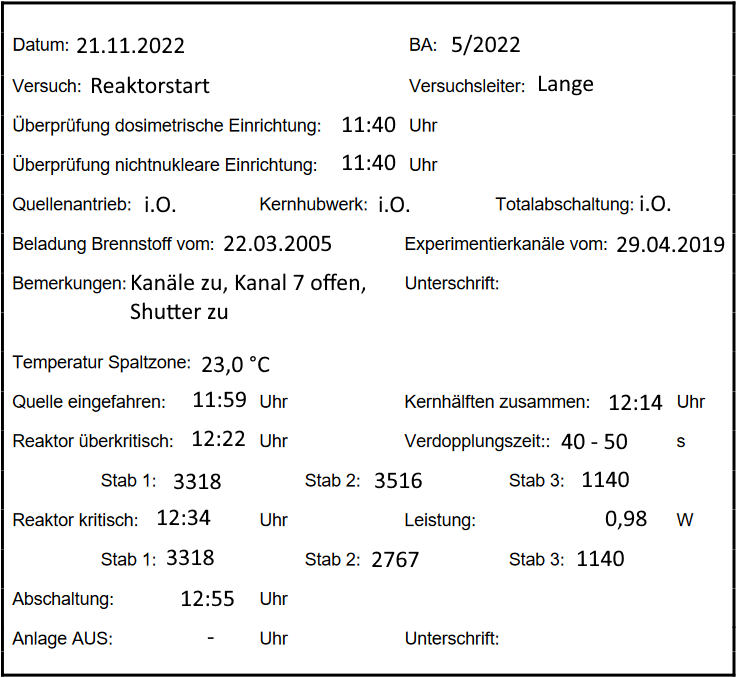
\includegraphics{BJ_Reaktorstart.png}
	
	\newpage
	
	\section{Protokoll des Anlassvorgangs}
	\begin{enumerate}
		\item Einfahren der Anfahrneutronenquelle
		\item Heben der unteren Kernhälfte mittels Kernhubwerk
		\item Einschalten des Anlassschalters
		\item Einzelnes Ausfahren der Steuerstäbe bis Erreichen des überkritischen Zustandes
		\item Überwachen des Leistungsanstieges bis ca. 1 Watt
		\item Schrittweises Einfahren der Steuerstäbe bis Erreichen des kritischen Zustandes bei einer Leistungsabgabe von 1 Watt
	\end{enumerate}

	\section{Kritische Stabstellung als Funktion der Leistung}
	\begin{table}[htpb]
		\begin{tabularx}{\textwidth}{X|X|X|X}
			Leistung & Stabstellung 1 & Stabstellung 2 & Stabstellung 3 \\
			\hline
			1 W & 3318 & 2767 & 1140 \\
			2 W & 3318 & 2846 & 1144
		\end{tabularx}
		\caption{Stellung der Steuerstäbe}
	\end{table}

	\noindent
	\textbf{Messunsicherheiten:}
	\begin{itemize}
		\item Steuerstabsposition nicht exakt bei 1 und 2 W abgelesen
		\item Keine exakte Bestimmung der Reaktivität möglich, dadurch Ungenauigkeiten bei Steuerstabspositionen
	\end{itemize}

	\noindent
	\textbf{Auswertung der Messergebnisse:} \\
	Kritische Stabstellung ist nahezu konstant, damit unabhängig von Reaktorleistung

	\section{Bestimmung der Gamma-Dosisleistung als Funktion der Reaktorleistung}
	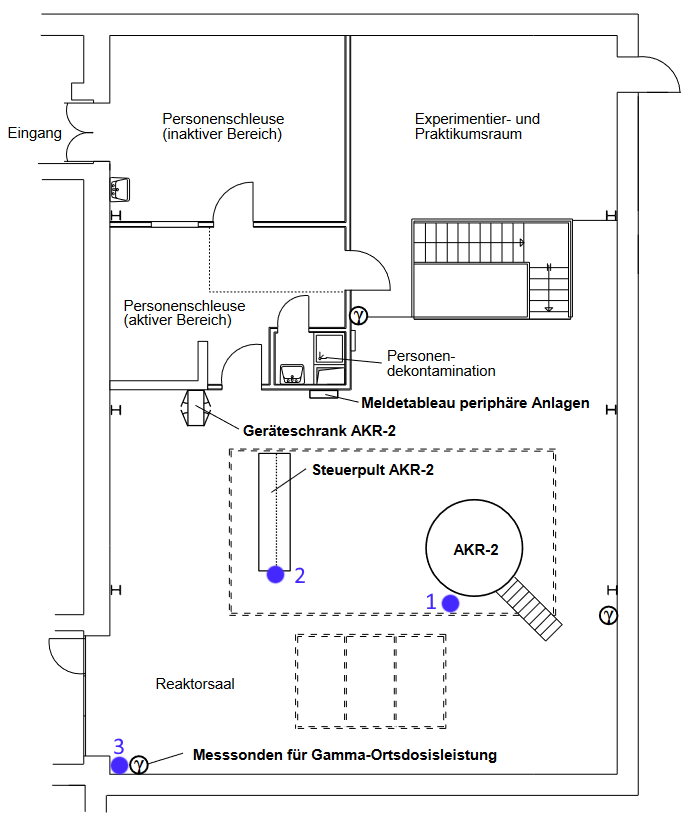
\includegraphics{AKR_Raumplan_Messpunkte.png}
	\begin{enumerate}
		\item Oberfläche Reaktor (0 Meter)
		\item Steuerpult (3 Meter)
		\item Ecke des Raums (9 Meter)
	\end{enumerate}

	\begin{table}[htpb]
		\begin{tabularx}{\textwidth}{X|X|X|X|X}
			\toprule
			\textbf{Messpunkt} & \multicolumn{2}{c}{\textbf{Gamma}} & \multicolumn{2}{c}{\textbf{Neutronen}} \\
			\cmidrule{2-3}\cmidrule{4-5}
			& 1 W & 2 W & 1 W & 2 W \\
			\midrule
			1 (0 m) & $15\: \mu Sv / h$ & $20\: \mu Sv / h$ & $1,8\: \mu Sv / h$ & $5\: \mu Sv / h$ \\
			2 (3 m) & $1\: \mu Sv / h$ & $2,5\: \mu Sv / h$ & $0,16\: \mu Sv / h$ & $0,7\: \mu Sv / h$ \\
			3 (9 m) & $0,2\: \mu Sv / h$ & $0,6\: \mu Sv / h$ & $0,12\: \mu Sv / h$ & $0,1\: \mu Sv / h$ \\
			\bottomrule
		\end{tabularx}
		\caption{Gamma- und Neutronen-Dosisleistung}
	\end{table}

	\begin{figure}[htpb]
		\begin{minipage}[t]{0.4\textwidth}
			\begin{tikzpicture}
				\begin{axis}[
					xlabel=$Abstand\: vom\: Reaktor (m)$,
					ylabel=$\mu Sv / h$,
					xmin=-1, xmax=10,
					ymin=0, ymax=22,
					xtick={0,3,9},
					xticklabels={0,3,9},
					ytick={0,2,...,22}
				]
					\addplot[mark=*, blue] plot coordinates {
						(0,15)
						(3,1)
						(9,0.2)
					};
					\addlegendentry{1 Watt Gamma}
					
					\addplot[mark=x, red] plot coordinates {
						(0,20)
						(3,2.5)
						(9,0.6)
					};
					\addlegendentry{2 Watt Gamma}
				\end{axis}
			\end{tikzpicture}
		\end{minipage}
		\hfill
		\begin{minipage}[t]{0.4\textwidth}
			\begin{tikzpicture}
				\begin{axis}[
					xlabel=$Abstand\: vom\: Reaktor (m)$,
					ylabel=$\mu Sv / h$,
					xmin=-1, xmax=10,
					ymin=0, ymax=6,
					xtick={0,3,9},
					xticklabels={0,3,9},
					ytick={0,1,...,6}
				]
					\addplot[mark=*,blue] plot coordinates {
						(0,1.8)
						(3,0.16)
						(9,0.12)
					};
					\addlegendentry{1 Watt Neutronen}
					
					\addplot[mark=x,red] plot coordinates {
						(0,5)
						(3,0.7)
						(9,0.1)
					};
					\addlegendentry{2 Watt Neutronen}
				\end{axis}
			\end{tikzpicture}
		\end{minipage}
	\end{figure}

	\noindent
	\textbf{Auswertung der Messergebnisse:} \\
	Die Dosisleistung verhält sich augenscheinlich invers proportional zum Abstand vom Reaktor. \\
	Bei höherer Reaktorleistung kommt es auch zu höheren Dosisleistungen. \\
	Es gibt stets eine geringere Neutronen-Dosisleistung als die Gamma-Dosisleistung.
\end{document}